\documentclass[12pt]{beamer}

\usetheme{Air}
\usepackage{thumbpdf}
\usepackage{wasysym}
\usepackage{ucs}
\usepackage[utf8]{inputenc}
\usepackage{pgf,pgfarrows,pgfnodes,pgfautomata,pgfheaps,pgfshade}
\usepackage{verbatim}
\usenavigationsymbolstemplate{}

\pdfinfo
{
  /Title       (KDE)
  /Creator     (LATEX)
  /Author      (RAFAEL FERNANDEZ LOPEZ)
}


\title{KDE}
\subtitle{Experience Freedom !}
\author{Rafael Fernández López}
\date{Julio, 2010}

\begin{document}

\begin{frame}{Party Quijote 2010}
  \framesubtitle{ereslibre@kde.org}
  \titlepage
\end{frame}

\section*{}
\begin{frame}
  \frametitle{Party Quijote 2010}
  \tableofcontents[section=1,hidesubsections]
\end{frame}

\AtBeginSection[]
{
  \frame<handout:0>
  {
    \frametitle{Party Quijote 2010}
    \tableofcontents[currentsection,hideallsubsections]
  }
}

\newcommand<>{\highlighton}[1]{%
  \alt#2{\structure{#1}}{{#1}}
}

\newcommand{\icon}[1]{\pgfimage[height=1em]{#1}}

%%%%%%%%%%%%%%%%%%%%%%%%%%%%%%%%%%%%%%%%%
%%%%%%%%%% Content starts here %%%%%%%%%%
%%%%%%%%%%%%%%%%%%%%%%%%%%%%%%%%%%%%%%%%%

\section{¿Qué es KDE?}

\begin{frame}{¿Qué es KDE?}
    \framesubtitle{Intento 1º}
    \center
    \begin{figure}
        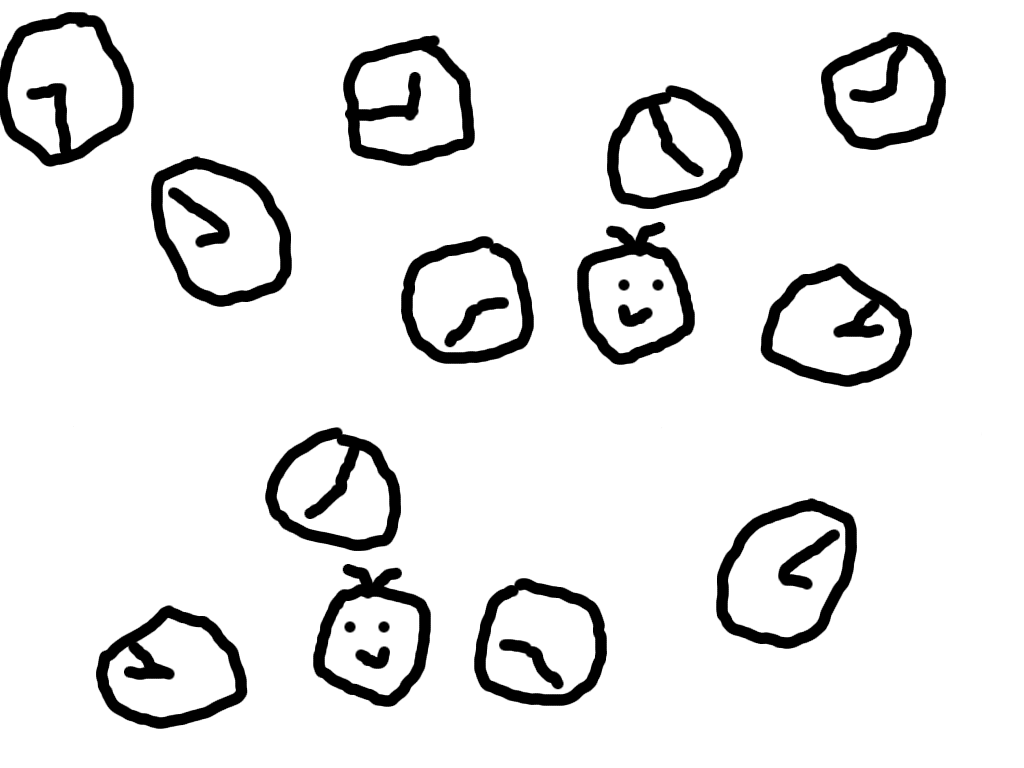
\includegraphics[width=9cm]{kde40.png}
    \end{figure}
\end{frame}

\begin{frame}{¿Qué es KDE?}
    \framesubtitle{Intento 2º}
    \center
    \begin{figure}
        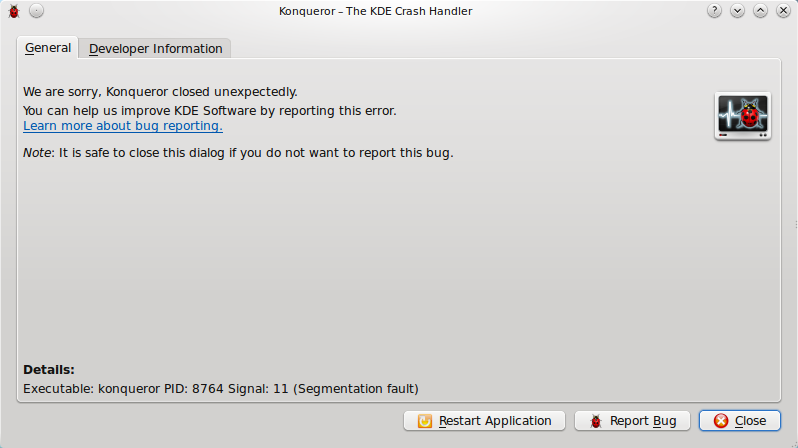
\includegraphics[width=9cm]{snapshot3.png}
    \end{figure}
\end{frame}

\begin{frame}{¿Qué es KDE?}
    \framesubtitle{Intento 3º (a la tercera...)}
    \begin{itemize}
        \item Comunidad
        \pause
        \begin{itemize}
            \item Programadores
            \item Artistas
            \item Traductores
            \item Documentadores
            \item Sysadmins
            \item Marketing (bloggers...)
            \item Diseñadores web
            \item Soporte
            \item ...
        \end{itemize}
        \pause
        \item Una gran familia
    \end{itemize}
\end{frame}

\section{Orígenes}

\begin{frame}{KDE 4.0}
    \center
    \begin{figure}
        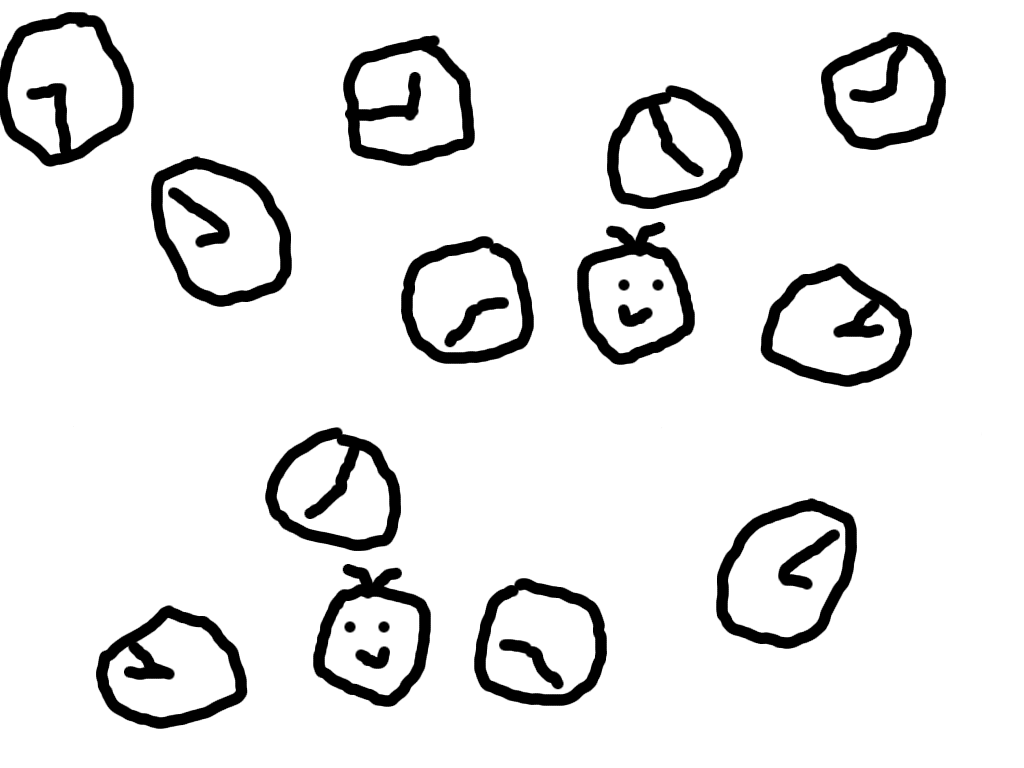
\includegraphics[width=9cm]{kde40.png}
    \end{figure}
\end{frame}

\begin{frame}{KDE 4.0}
    \center
    \begin{figure}
        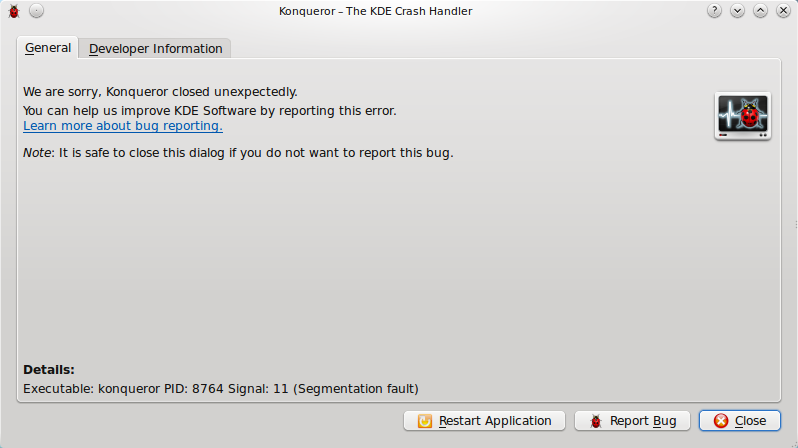
\includegraphics[width=9cm]{snapshot3.png}
    \end{figure}
\end{frame}

\begin{frame}{Entorno}
    \begin{itemize}
        \item Compilación
        \begin{itemize}
            \item Autohell $\rightarrow$ CMake
        \end{itemize}
        \bigskip
        \item Protocolo de Intercomunicación entre Procesos (IPC)
        \begin{itemize}
            \item DCOP $\rightarrow$ D-Bus
        \end{itemize}
    \end{itemize}
\end{frame}

\begin{frame}{Plataformas}
    \begin{itemize}
        \item Qt 4.0
        \item Plasma
        \item Solid
        \item Phonon
        \item Nepomuk
        \item Strigi
        \item Sonnet
        \item Akonadi
        \item ThreadWeaver
        \item Raptor
        \item Kross
    \end{itemize}
\end{frame}

\begin{frame}{KDE 4.1 $\rightarrow$ KDE 4.$\infty$}
    \center
    \begin{figure}
        
\includegraphics[width=8cm]{cat.jpg}
    \end{figure}
\end{frame}

\section{Actualidad}

\begin{frame}{KDE SC 4.4}
    \begin{itemize}
        \item Estable
        \bigskip
        \item Potente
        \bigskip
        \item Elegante
        \bigskip
        \item Bonito
    \end{itemize}
\end{frame}

\section{Futuro}

\begin{frame}{KDE SC 4.5 $\rightarrow$ KDE SC 4.x, $x \ge 6$}
    \center
    \begin{figure}
        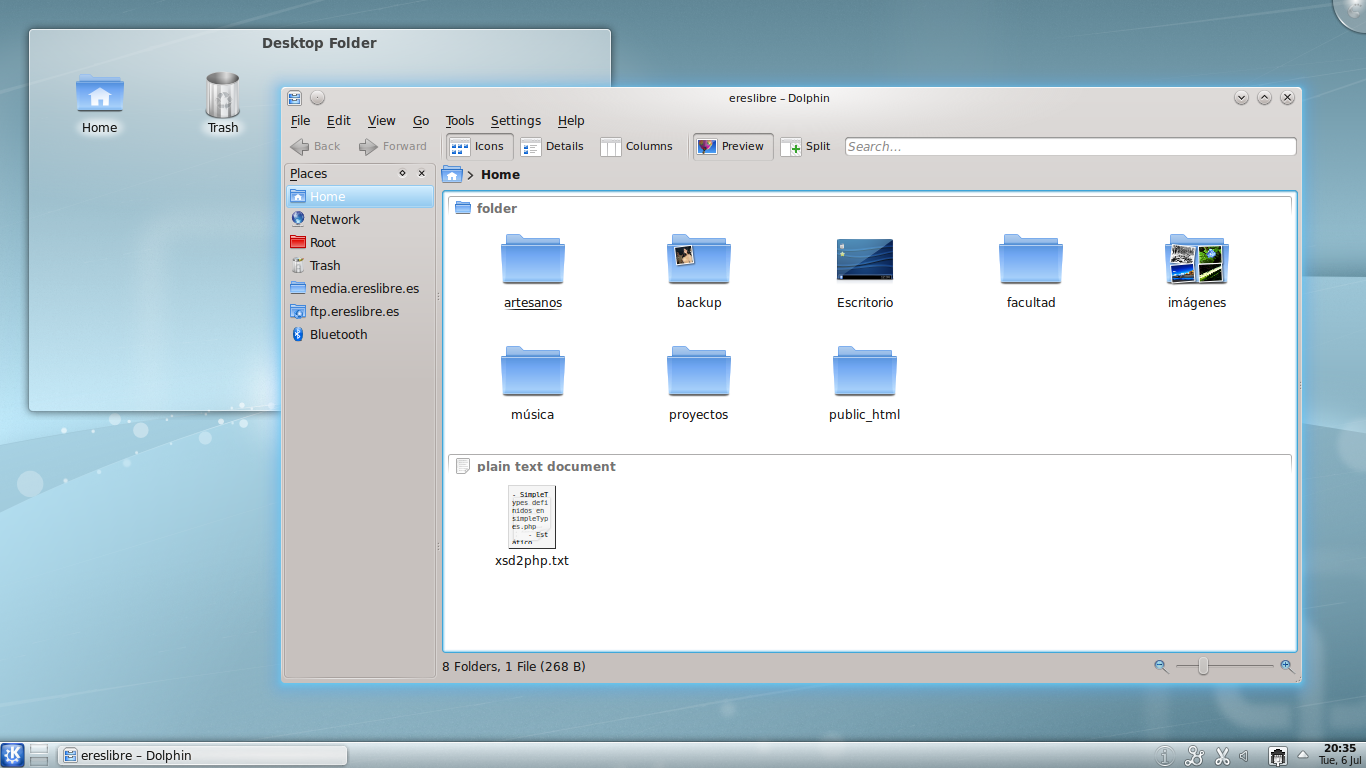
\includegraphics[width=11cm]{kde45.png}
    \end{figure}
\end{frame}

\begin{frame}{KDE SC 4.5 $\rightarrow$ KDE SC 4.x, $x \ge 6$}
    \center
    \begin{itemize}
        \item Continuar estabilización
        \bigskip
        \item Traducción completa
        \bigskip
        \item Documentación
        \bigskip
        \item Experiencia del usuario
        \bigskip
        \item KDE en:
        \begin{itemize}
            \item Tostadoras
            \item Lavadoras
            \item ...
        \end{itemize}
    \end{itemize}
\end{frame}

\begin{frame}{KDE SC 4.5 $\rightarrow$ KDE SC 4.x, $x \ge 6$}
    \center
    \begin{figure}
        
\includegraphics[width=8cm]{cat.jpg}
    \end{figure}
\end{frame}

\frame{
  \frametitle{Party Quijote 2010}
  \vspace{1.5cm}
  {\huge \alert{\textbf{Gracias.}} ¿Preguntas?}

  \vspace{1cm}
  \begin{center}
    \large \textbf{http://www.kde.org/}
  \end{center}


  \vspace{1cm}
  \begin{flushright}
    Rafael Fernández López

    \structure{\footnotesize{ereslibre@kde.org}}
  \end{flushright}
}

\end{document}
